\label{ch:symmetry}

\section{Cayley diagram}
\label{sec:cayley-diagram}

We have seen in the previous chapter how cyclic groups
(those generated by a single generator)
have neatly described torsors.

In this section we shall generalize this story
to groups $G$ generated by a
(finite or just decidable)
set of generators $S$.

\tikzset{vertex/.style={circle,fill=black,inner sep=0pt,minimum size=4pt}}
\tikzset{gena/.style={draw=blue!70,-stealth}}
\tikzset{genb/.style={draw=red!70,-stealth}}

\begin{figure}
  \centering
  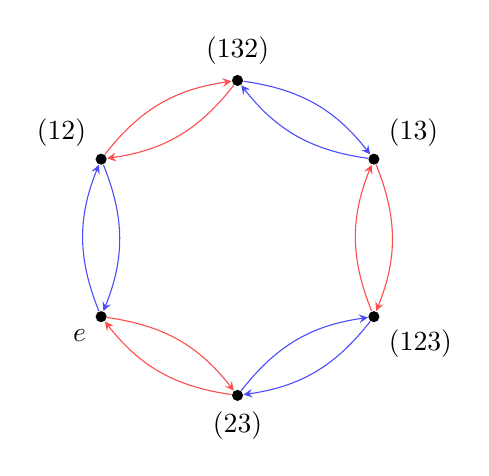
\begin{tikzpicture}
    \pgfmathsetmacro{\len}{2}
    \node[vertex,label=30:$(13)$]   (n13)  at (30:\len)  {};
    \node[vertex,label=90:$(132)$]  (n132) at (90:\len)  {};
    \node[vertex,label=150:$(12)$]  (n12)  at (150:\len) {};
    \node[vertex,label=210:$e$]     (ne)   at (210:\len) {};
    \node[vertex,label=270:$(23)$]  (n23)  at (270:\len) {};
    \node[vertex,label=330:$(123)$] (n123) at (330:\len) {};
    \begin{scope}[every to/.style={bend left=22}]
      % generator a is (12)
      \draw[gena] (ne)   to (n12);
      \draw[gena] (n12)  to (ne);
      \draw[gena] (n13)  to (n132);
      \draw[gena] (n132) to (n13);
      \draw[gena] (n123) to (n23);
      \draw[gena] (n23)  to (n123);
      % generator b is (23)
      \draw[genb] (ne)   to (n23);
      \draw[genb] (n23)  to (ne);
      \draw[genb] (n13)  to (n123);
      \draw[genb] (n123) to (n13);
      \draw[genb] (n12)  to (n132);
      \draw[genb] (n132) to (n12);
    \end{scope}
  \end{tikzpicture}
  \caption{Cayley diagram for $S_3$ with respect to $S = \{(12),(23)\}$.}
  \label{fig:cayley-s3}
\end{figure}

$G \equiv \Aut(D_G) \to \Sym(\Card G)$

\section{Actions}
\label{sec:actions}

If $G$ is any (possibly higher) group and $A$ is any type of objects,
then we define an \emph{action} by $G$ in the world of elements of $A$ as a function
\[
  X : \B G \to A.
\]
The particular $A$ being acted on is $X(\pt):A$,
and the action itself is given by transport.
This generalizes our earlier definition of $G$-sets, $X : \B G \to \Set$.

Notice that the type $\B G \to A$ is equivalent to the type
\[
  \sum_{a:A}\hom(G,\Aut_A(a)),
\]
that is, the type of pairs of an element $a : A$,
and a homomorphism from $G$ to the automorphism group of $A$.
The equivalence maps $X:\B G\to A$ to the pair consisting of $X(\pt)$
and the homomorphism represented by the pointed map arising
from corestricting $X$ to factor through the component of $A$ containing $a$
together with the trivial proof that this map takes $\pt:\B G$ to $a$.

Because of this equivalence,
we define a \emph{$G$-action on $a:A$}
to be a homomorphism from $G$ to $\Aut_A(a)$.

Many times we are particularly interested in actions on types,
i.e., $A$ is a universe (or the universe of types-at-large):
\[
  X : \B G \to \Type.
\]

In this case, we define \emph{orbit type} of the action as
\[
  X_G \defeq \sum_{z:\B G} X(z),
\]
and the type of \emph{fixed points} as
\[
  X^G \defeq \prod_{z:\B G} X(z).
\]
The set of orbits is the set-truncation of the orbit type,
\[
  X / G \defeq \Trunc{X_G}_0.
\]
We say that the action is \emph{transitive} if $X / G$ is contractible.

\section{Semidirect products}
\label{sec:Semidirect-products}

\begin{definition}\label{def:semidirect-product}
  Given a group $G$ and an action $\tilde H : BG \to \typegroup$ on a group $H \defeq \tilde H(\pt)$, we define a group called the {\em
    semidirect product}
  $G \ltimes H$ to be the total space
  $$\Bop ( G \ltimes H ) \defeq \sum_{t:\B G} \B \tilde H(t)$$
  equipped with the point $(\pt,\pt)$ as basepoint and equipped with a proof that it is a connected groupoid.
\end{definition}

The notation $G \ltimes H$, following standard practice, is an abuse, because it includes no reference to the action $\tilde H$, which is needed
to perform the construction.

FILL IN SOME FACTS ABOUT PATHS ON TOTAL SPACES BEING PAIRS OF PATHS, INCLUDING WHAT PATH COMPOSITION LOOKS LIKE IN TERMS OF THOSE PAIRS.

\begin{exercise}
  Construct a section of the projection $ \Bop ( G \ltimes H ) \to \B G $ by sending $t$ to $(t,pt)$.
  Construct an equivalence between the set $\abstrOp (G \ltimes H)$ and the set $\abstrOp G \times \abstrOp H$.  Use the equivalence to work out
  explicit formulas for multiplication and for the inverse operation in the abstract group $\abstrOp (G \ltimes H)$.
\end{exercise}

\section{Orbit-stabilizer theorem}
\label{sec:orbit-stabilizer-theorem}

Given an action $X : \B G \to \Type$ and a point $x : X(\pt)$, we define
the \emph{orbit} through $x$ as the subtype of $X(\pt)$ consisting of
all $y : X(\pt)$ that are merely equal to $x$ in the orbit type:
\[
  G\cdot x \defeq \mathcal O_x \defeq \sum_{y : X(\pt)} \merely{[x] = [y]}
\]
(Note the unfortunate terminology: an orbit is not an element in the
orbit type!)
Note that this only depends on the image of $x$ in the set of orbits,
thus justifying the names.

In this way, the type $X(\pt)$ splits as a disjoint union of orbits,
indexed by the set of orbits
\[
  X(\pt) \equiv \coprod_{z : X / G} \mathcal O_z.
\]

The \emph{stabilizer group} $G_x$ of $x : X(\pt)$ is the automorphism group of $[x]$ in the orbit type.
Different points in the same orbit have conjugate stabilizer groups.

We say that the action is \emph{free} if all stabilizer groups are trivial.

\begin{theorem}[Orbit-stabilizer theorem]
  Fix a $G$-type $X$ and a point $x : X(\pt)$.
  There is a canonical action $\tilde G : \B G_x \to \Type$,
  acting on $\tilde G(\pt)\equiv G$
  with orbit type $\tilde G\dblslash G_x \equiv \mathcal O_x$.
\end{theorem}
\begin{proof}
  Define $\tilde G(x,y,!) \defeq (\pt = x)$.
\end{proof}

Now suppose that $G$ is a $1$-group acting on a set.
We see that the orbit type is a set
(and is thus equivalent to the set of orbits)
if and only if
all stabilizer groups are trivial,
\ie if and only if the action is free.

If $G$ is a $1$-group,
then so is each stabilizer-group,
and in this case (of a set-action),
the orbit-stabilizer theorem
tells us that 

\begin{theorem}[Lagrange's Theorem]
  If $H \to G$ is a subgroup, then $H$ has a natural action on $G$,
  and all the orbits under this action are equivalent.
\end{theorem}

% Interaction with cardinality: if G acts freely on S, then card(S/G) = card(S)/card(G)

\section{The isomorphism theorems}
\label{sec:noether-theorems}

First a remark about maps between groupoids.
Let $f : X \to Y$, and write $f$ as a projection from a sigma-type:
$\sum_{y:Y} f^{-1}(y) \to Y$,
projecting away the fibers $f^{-1}(y)$.
We say that $f$ \emph{forgets} these fibers.
In general, the fibers are themselves groupoids,
but it can happen that they are sets, propositions, or even contractible.
Accordingly, we say that:
\begin{itemize}
\item $f$ \emph{forgets at most structure} if all the fibers are sets;
\item $f$ \emph{forgets properties} if all the fibers are propositions;
\item $f$ \emph{forgets nothing} if all the fibers are contractible.
\end{itemize}
(Of course, in the latter case, $f$ is an equivalence.)

We can factor $f$ through its $0$- and $-1$-image as follows:
\[
  \sum_{y:Y} f^{-1}(y) \to
  \sum_{y:Y} \Trunc{f^{-1}(y)}_0 \to
  \sum_{y:Y} \Trunc{f^{-1}(y)}_{-1} \to
  \sum_{y:Y} \Trunc{f^{-1}(y)}_{-2} = Y.
\]
Here, the first map \emph{forgets stuff} (it is $0$-connected),
the second map \emph{forgets structure} (it is a $-1$-connected set map),
while the last \emph{forgets properties}.

For example, the inclusion of the type of sets with cardinality
$n$ into the type of all finite sets
forgets properties.

Group homomorphisms provide examples of forgetting stuff and structure.
For example, the map from cyclically ordered sets with cardinality $n$
to the type of sets with cardinality $n$ forgets structure,
and represents an injective group homomorphism from the cyclic
group of order $n$ to the symmetric group $\Sigma_n$.

And the map from pairs of $n$-element sets to $n$-element sets
that projects onto the first factor clearly forgets stuff,
namely, the other component.
It represents a surjective group homomorphism.

More formally, fix two groups $G$ and $H$,
and consider a homomorphism $\varphi$ from $G$ to $H$,
considered as a pointed map $\B\varphi : \B G \to_\pt \B H$.
Then $\B\varphi$ factors as
\begin{align*}
  \B G
  = &\sum_{w:\B H}\sum_{z:\B G}(\B\varphi(z)=w)\\
  \to_\pt &\sum_{w:\B H}\Trunc*{\sum_{z:\B G}(\B\varphi(z)=w)}_0\\
  \to_\pt &\sum_{w:\B H}\Trunc*{\sum_{z:\B G}(\B\varphi(z)=w)}_{-1} = \B H.
\end{align*}
The pointed, connected type in the middle represents a group
that is called the \emph{image} of $\varphi$, $\Img(\varphi)$.

(FIXME: Quotient groups as automorphism groups, normal subgroups/normalizer, subgroup lattice)


\section{(the lemma that is not) Burnside's lemma}
\label{sec:burnsides-lemma}

% Where does this go?!
\section{More about automorphisms}
\label{sec:automorphisms}

% Written to record somewhere the results of a discussion with Bjorn
For every group $G$ (which for the purposes of the discussion
in this section we allow to be a higher group)
we have the automorphism group $\Aut(G)$.
This is of course the group of self-identifications $G = G$ in the type of groups, $\Group$.
If we represent $G$ by the pointed connected classifying type $\B G$,
then $\Aut(G)$ is the type of pointed self-equivalences of $\B G$.

We have a natural forgetful map from groups to the type of connected groupoids.
Define the type $\Bunch$ to be the type of all connected groupoid.
If $X:\Bunch$, then all the elements of $X$ are merely isomorphic,
that is, they all look alike,
so it makes sense to say that $X$ consists of a \emph{bunch} of alike objects.

For every group $G$ we have a corresponding bunch, $\B G_\div$,
\ie{} the collection of $G$-torsors,
and if we remember the basepoint $\pt : \B G_\div$,
then we recover the group $G$.
Thus, the type of groups equivalent to the type
$\sum_{X : \Bunch} X$
of pairs of a bunch together with a chosen element.
(This is essentially our definition of the type $\Group$.)

Sometimes we want to emphasize that we $\B G_\div$ is a bunch,
so we define $\bunch(G) \defeq \B G_\div : \Bunch$.

\begin{definition}[The center as an abelian group]
  Let $Z(G) \defeq \prod_{z : \B G}(z = z)$ denote the type of fixed points of the adjoint action of $G$ on itself.
  This type is equivalent to the automorphism group of the identity on $\bunch(G)$,
  and hence the loop type of
  \[
    \B Z(G) \defeq \sum_{f : \B G \to \B G} \merely{f \sim \id}.
  \]
  This type is itself the loop type of the pointed, connected type
  \[
    \B^2Z(G) \defeq \sum_{X : \Bunch}\Trunc{\bunch(G) = X}_0,
  \]
  and we use this to give $Z(G)$ the structure of an \emph{abelian} group,
  called the \emph{center} of $G$.
\end{definition}
There is a canonical homomorphism from $Z(G)$ to $G$ given by the pointed map
from $\B Z(G)$ to $\B G$ that evaluates at the point $\pt$.
The fiber of the evaluation map $e : \B Z(G) \to_\pt \B G$ is
\begin{align*}
  \fiber_e(\pt)
  &\jdeq \sum_{f : \B G \to \B G} \merely{f \sim \id} \times (\mathop f \pt = \pt) \\
  &\equiv \sum_{f : \B G \to_\pt \B G} \merely{f \sim \id},
\end{align*}
and this type is the loop type of the pointed, connected type
\[
  \B\Inn(G) \defeq \sum_{H : \Group} \Trunc{\bunch(G) = \bunch(H)}_0,
\]
thus giving the homomorphism $Z(G)$ to $G$ a normal structure with
quotient group $\Inn(G)$, called the \emph{inner automorphism group}.

Note that there is a canonical homomorphism from $\Inn(G)$ to $\Aut(G)$
given by the pointed map $i : \B\Inn(G) \to \B\Aut(G)$ that forgets the component.
On loops, $i$ gives the inclusion into $\Aut(G)$ of the subtype of automorphisms of $G$
that become merely equal to the identity automorphism of $\bunch(G)$.
The fiber of $i$ is
\begin{align*}
  \fiber_i(\pt)
  &\jdeq \sum_{H : \Group} \Trunc{\bunch(G) = \bunch(H)}_0 \times (H = G) \\
  &\equiv \Trunc{\bunch(G) = \bunch(G)}_0.
\end{align*}
This is evidently the type of loops in the pointed, connected groupoid
\[
  \B\Out(G) \defeq \Trunc*{\sum_{X : \Bunch}\merely{\bunch(G) = X}}_1,
\]
thus giving the homomorphism $\Inn(G)$ to $\Aut(G)$ a normal structure with
quotient group $\Out(G)$, called the \emph{outer automorphism group}.
Note that $\Out(G)$ is always a $1$-group,
and that it is the decategorification of $\Aut(\bunch(G))$.

\begin{theorem}
  Let two groups $G$ and $H$ be given.
  There is a canonical action of $\Inn(H)$
  on the set of homomorphisms from $G$ to $H$, $\Trunc{\B G \to_\pt \B H}_0$.
  This gives rise to an equivalence
  \[
    \Trunc{\B G_\div \to \B H_\div}_0 \equiv \Trunc*{\Trunc{\B G \to_\pt \B H}_0 \dblslash \Inn(H)}_0
  \]
  between the set of maps from $\bunch(G)$ to $\bunch(H)$ and the set of
  components of the orbit type of this action.
\end{theorem}
\begin{proof}
  We give the action by defining a type family $X : \B\Inn(H) \to \Type$ as follows
  \[
    X\, \angled{K,\phi} \defeq \Trunc{\Hom(G,K)}_0 \jdeq \Trunc{\B G \to_\pt \B K}_0,
  \]
  for $\angled{K,\phi} : \B\Inn(H) \jdeq \sum_{K : \Group} \Trunc{\bunch(H) = \bunch(K)}_0$.
  Now we can calculate
  \begin{align*}
    \Trunc{X_{\Inn(H)}}_0
    &\jdeq \Trunc*{\sum_{K:\Group}\Trunc{\bunch(H)=\bunch(K)}_0\times\Trunc{\Hom(G,K)}}_0 \\
    &\equiv \Trunc*{\sum_{K:\Group}(\bunch(H)=\bunch(K))\times\Hom(G,K)}_0 \\
    &\equiv \Trunc*{\sum_{K:\Bunch}\sum_{k:K}(\bunch(H)=K)\times\sum_{f:\bunch(G)\to K)}\mathop f \pt = k}_0 \\
    &\equiv \Trunc*{\sum_{K:\Bunch} (\bunch(H)=K) \times(\bunch(G) \to K)}_0 \\
    &\equiv \Trunc*{\bunch(G)\to\bunch(H)}_0 \jdeq \Trunc*{\B G_\div \to \B H_\div}_0.\qedhere
  \end{align*}
\end{proof}

%%% Local Variables:
%%% mode: latex
%%% fill-column: 144
%%% TeX-master: "book"
%%% End:
